\documentclass[a4paper,11pt]{article}
\usepackage[latin1]{inputenc}
%\usepackage[danish]{babel}
\usepackage[pdftex]{graphicx}
\usepackage{epstopdf}
%\usepackage[dvips] {graphicx}
\usepackage[mathcal]{euscript}
\usepackage{epsfig}
\usepackage[]{amsmath}
%\usepackage{empheq07}		% to put box around aling sequence (replacing eqnarray}
\usepackage{fancyhdr}
%\usepackage{here}
\usepackage{rotating}
\usepackage{lscape}
%\usepackage{hyperref}
%\usepackage{pdfpages}		%enables the insert of other pdf documents
\usepackage{natbib}	%enables the use of \citep and others; see http://merkel.zoneo.net/Latex/natbib.php
\usepackage{amsfonts,amssymb,latexsym,epsfig,color}

	\addtolength{\oddsidemargin}{-.875in}
	\addtolength{\evensidemargin}{-.875in}
	\addtolength{\textwidth}{1.95in}
	\addtolength{\topmargin}{-1.175in}
	\addtolength{\textheight}{1.75in}

% %% Turning references and citations into hyperlinks
 \usepackage{color}			      % using color package
 \definecolor{midgray}{gray}{0.4}		% defining gray color
 \usepackage[pdftex,colorlinks=true,citecolor=midgray,linkcolor=midgray]{hyperref}

% ============================================================================
\begin{document}



\title{Selecting Lens Candidates (via Variability)}


\author{Schmidt, et al.}
%\affil{$^{1}$ Max Planck Institut f\"ur Astronomie, K\"onigstuhl 17, D-69117 Heidelberg, Germany}

%\email{kschmidt@mpia.de}

%\date{September 30, 2009}

\maketitle

%========================================================================
\begin{abstract}

The selection of the lens candidates which will be observed with the ESO 2.2m and the GROND instrument on december 11-17 2010 is presented. The candidates consist of three kinds of objects: 1) Extended objects and 2) Spectroscopically confirmed QSOs from SDSS Stripe 82  selected via variability and their UV excess colors and 3) spectroscopically confirmed Stripe 82 quasars failing the variability+UVX selection but marked as 'personal favorites'. Each object has been assigned a priority ID. Based on these IDs 5 'personal favorites', 20 Stripe 82 QSOs (which are not in M. Oguri's catalogue of rejected lens candidates) and 362 extended UVX objects have been selected to be observed. Of these an estimated total of $\sim$200 objects will be observed with the time awarded.
\end{abstract}

%========================================================================
\section{Introduction}

In this short document the selection of the lens candidates which will be observed at La Silla in mid december 2010 is described. The purpose of this work is to identify the first lensed quasars selected based on the quasar's intrinsic variability. The idea is to look for unresolved lenses in SDSS Stripe 82 where the average time sampling (on average 60 epochs over 8 years) is good enough for a solid variability selection. The applied variability cut is described in detail in \cite{schmidt10}.

The total number of lensed QSOs expected in Stripe 82 ($i_\textrm{lim}=21.3$) is $\simeq 8$ \cite{oguri10}. Having shown in \cite{schmidt10} that the QSO selection algorithm approach 90\% completeness at $i > 19.5$, 5-7 of the selected candidates are expected to be confirmed as QSO lenses. So far only two lenses are known in Stripe 82 \citep{lacki08,jackson08} so any increase in the number of lenses with the time sampling of Stripe 82 is desirable. Furthermore, confirming {\it any} of the candidates as actual lenses will, despite previous efforts, be the first time that a gravitational lens has been selected based on variability.


%========================================================================
\section{Initial Samples}

Below we describe the initial data samples. It is these samples which have been cut down by color, variability, redshift, etc. to create the samples from which the objects to observe have been selected.

\subsection{Extended Objects}

The initial sample of extended objects was selected from Stripe 82 by asking for all objects with the SDSS DR7 type keyword set to 3, i.e., extended/galaxy morphology. This is done to look for unresolved small-separation lenses. The hope is that the lenses hide in the relatively poor SDSS seeing (which nevertheless goes down to $\sim0.7-0.8$ for the best seeing ($gri$) epochs in Stripe 82) and can be found on their QSO variability and their multiple point sources in great seeing follow-up. Furthermore the objects have been asked to satisfy the color cuts shown in table~\ref{tab:UVX} \citep[table~1 in ][]{schmidt10}, which is where the main QSO locus is located in color space, eliminating the majority of stellar contaminants. Furthermore the objects have a brightness of $17<i< 21$. This returned an initial sample of 39,657 objects.

%%%%%%%%%%%%%%%%%%%%%%%%%%%%%%%%%%%%%%%%
% \begin{table}[thbp]
\begin{table}[!h]
\centering{
\caption[The UVX Color Box]{The UV excess (UVX) color box.}
%\tablenote{note.}
\label{tab:UVX}
\begin{tabular}[c]{|rcl|}
\hline
-0.4  $<$& $u-g$ & $<$ 0.6\\ 
-0.5  $<$& $g-r$ & $<$ 0.7 \\
-0.4  $<$& $r-i$ & $<$ 0.4 \\
%17 $<$ & $i$ & $<$ 21 \\
%290 deg  $<$& RA& $<$ 60 deg \\
%-1.25 deg  $<$& Dec & $<$ 1.25 deg \\
\hline
\end{tabular}}
\end{table}
%%%%%%%%%%%%%%%%%%%%%%%%%%%%%%%%%%%%%%%%

\subsection{Spectroscopically Confirmed SDSS Stripe 82 QSOs}

The initial sample of spectroscopically confirmed QSOs used here is the sample
of the 9157 quasars described in \cite{schmidt10}. This sample correspond to
all spectroscopically confirmed quasars in the DR5 QSO catalog
\citep{schneider07} located in Stripe 82.


%========================================================================
\section{Candidate Selection}\label{sec:cansel}

From the initial samples described above a series of different cuts were
applied to select the most interesting candidates for spectroscopic follow-up.
The following cuts were applied:

\begin{itemize}

\item \textbf{\cite{schmidt10} variability cut}: The $A$ and $\gamma$ values
defined in \cite{schmidt10} has been calculated for each object. 93\% of the
9157 quasars (the cut it is defined based on them) and 2.6\% (1027 of 39,657)
of the extended objects survive this cut.

\item \textbf{Removing obvious non-quasars by visual inspection}: This has
only been done for the extended variability selected objects, since the
variability selection was developed on point sources and hence the
contaminants ('normal' AGN, defects, variable blue galaxies etc.) are not
understood as well for extended objects as for point sources.

\item \textbf{UV excess cut (table~\ref{tab:UVX}) on colors}

\item \textbf{$z_\textrm{spec}>1$ or $z_\textrm{phot}>1$ when
$z_\textrm{spec}$ is not available}: One of the major contaminants of
unresolved quasar lenses (extended quasar colored objects) are low redshift
quasars looking extended because of the host galaxy, hence the candidates need
to have an estimated redshift above 1.

\item \textbf{Extended morphology}: Last but not least the type keyword need
to be set to 3 (extended morphology) in the best seeing Stripe 82 epoch where
the $r$-band seeing has to be less than 0.9".


\end{itemize}

Having done this we were left with a sample of 362 out of 39,657 extended
variable UVX objects and 320 out of 9,157 spectroscopically confirmed QSOs.
The selection process is illustrated in figure~\ref{fig:lenssel}.

%====================================
%====================================
\begin{figure}[thbp]
        \centering  
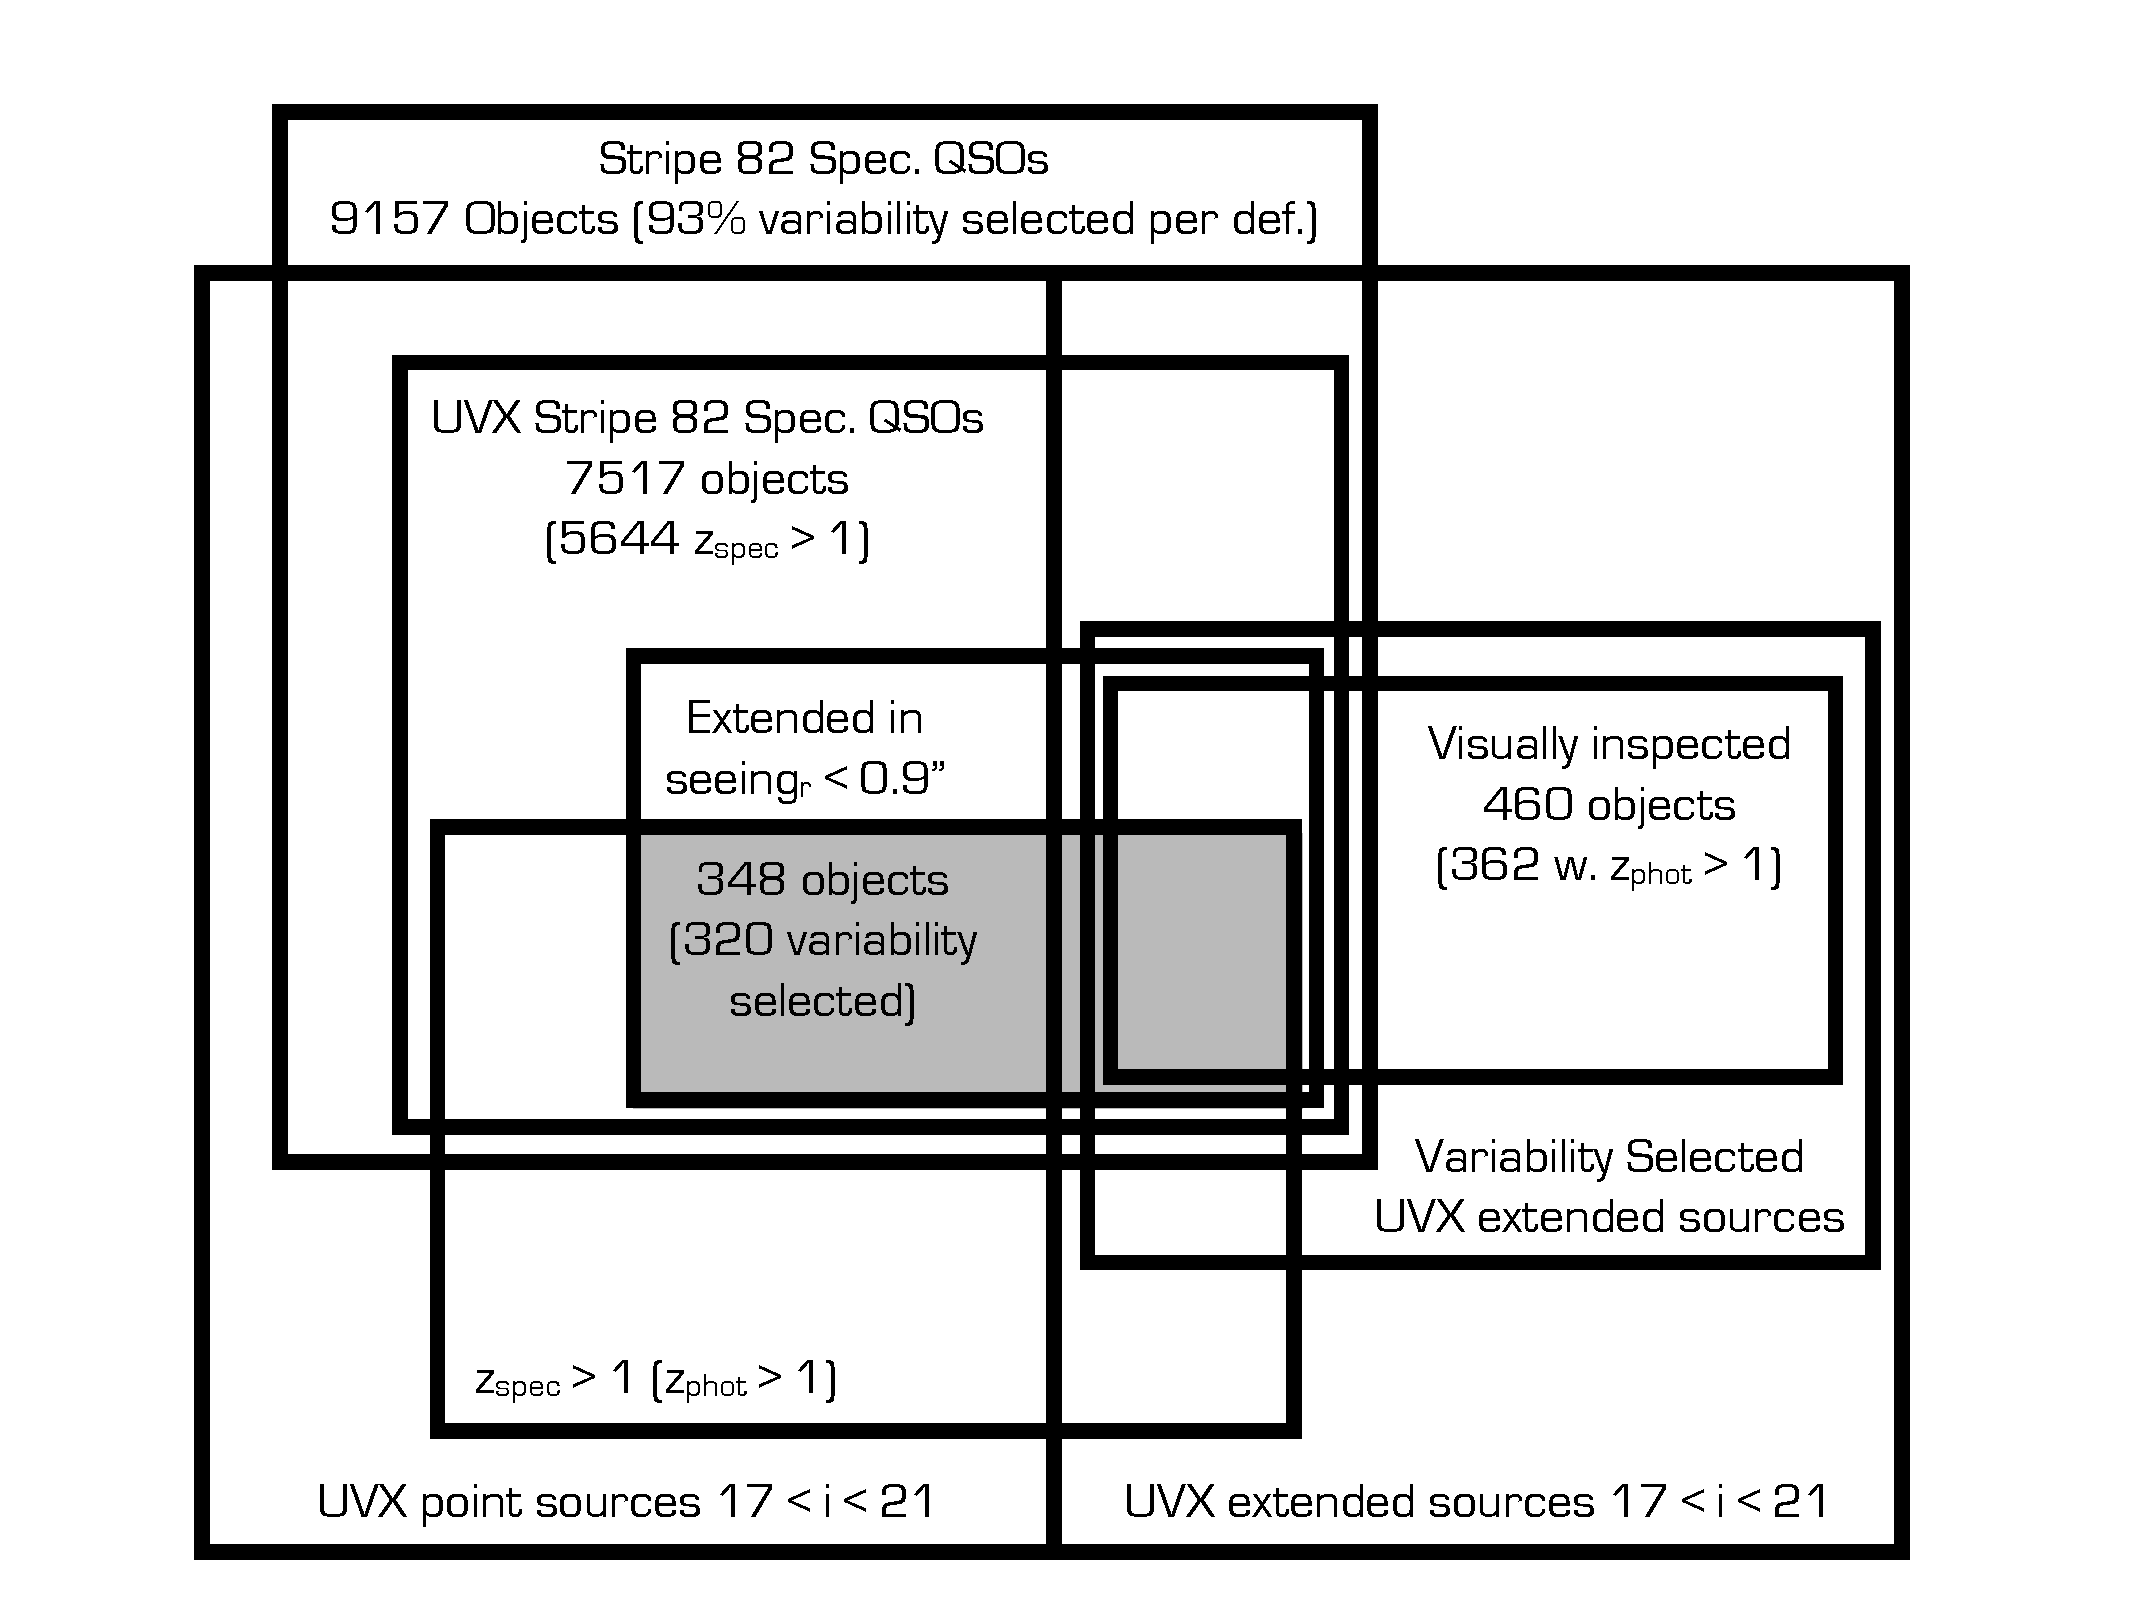
\includegraphics[width=0.90\textwidth]{figs/lenscandselection.pdf}
\textit{\caption[...]{Illustration of cuts made on the QSO and extended UVX sample as described in the text.}
\label{fig:lenssel}}
\end{figure} 
%====================================
%====================================


%========================================================================
\section{Priority ID}
Since we were not awarded enough time to observe all candidates they needed to
be prioritized. This was done by creating a 'priority ID' for each object on
which the observational order is based. The ID is simply a long (17 digits)
integer which indicates several 'properties' of the individual objects. The
priority IDs are created based on the following:
\begin{enumerate}

\item 'personal favorite'
\subitem This criterion is ranked higher than everything else, i.e., it vetoes
the observation of the given object by setting the first digit of the ID to 2.
The personal favorites selected here are described in a bit more detail in
section~\ref{sec:PF}

\item QSO spectrum  (with $z>1$) available
\subitem If a quasar spectrum with a redshift larger than 1 is available the
first digit of the ID is set to one.

\item UKIDSS H-band magnitude
\subitem In the case of cross-matched objects in UKIDSS the H-band magnitude
(or rather the maximum of all the H band magnitudes - 100 if not defined -
minus the individual magnitudes) is written to the next 4 digits with the dot
removed and two decimals.

\item  $\frac{\chi_\textrm{star}^2}{\chi_\textrm{phot}^2}$
\subitem This fraction estimates how 'close' the object is to the stellar
locus compared to the quasar locus in color-color space. The 'distances' to
the two loci is indicated by the $\chi_\textrm{star}^2$ and
$\chi_\textrm{phot}^2$ respectively. These are obtained when estimating the
photometric redshift of the object \citep[see][for more details]{hennawi10}.
The fraction is rounded of to nearest integer an occupies the next four
digits.

\item $z_\textrm{phot}$ 
\subitem The following 4 digits of the priority ID contains the photometric
redshift estimated as described in \cite{hennawi10} (dot removed and two
decimals).

\item $\frac{\textrm{type}_\textrm{gal}+1.0}{\textrm{type}_\textrm{star}+1.0}$
\subitem This fraction compares the number of epochs where the object was
flagged as extended ($\textrm{type}_\textrm{gal}$) with the number of epochs
where the object was point source like ($\textrm{type}_\textrm{star}$). The
fraction is rounded of to nearest integer an occupies the next four digits.

\end{enumerate}

Thus for a given object the priority ID might be 18142001518520018 corresponding to:\\
- A QSO spectrum with $z>1$ (and not a 'personal favorite'): \hfill \textbf{1}8142001518520018 \\
- A UKIDSS H-band magnitude of 100-81.42 = 18.58:  \hfill 1\textbf{8142}001518520018 \\
- 15 times 'closer' to the quasar locus than the stellar locus \hfill 18142\textbf{0015}18520018\\
- An estimated photometric redshift of 1.852: \hfill 181420015\textbf{1852}0018 \\
- 18 times as many Stripe 82 epochs with galaxy morphology (type = 3) than \\
 epochs where the object is point source like (type = 6): \hfill 1814200151852\textbf{0018}

Hence a large priority ID gives the object a high priority.

One flaw or limitation with this kind of priority ID is that each property
contributes to the ID independently, meaning that a lower ranked property is
only effective if several objects has the same values of the higher ranked
property(ies); for instance the $\chi^2$ criteria is effectively only used
when no H-band magnitude is known (or if two or more objects have the same
H-band magnitude to within a percent).

%========================================================================
\section{The final sample for GROND follow-up}

By creating the priority ID for each object in the samples resulting from the cuts described in section~\ref{sec:cansel}, we were now able to make the final list of objects to observe. We decided to select 5 'personal favorites' which didn't pass all cuts (more about these below), the 20 spectroscopically confirmed QSOs with the highest priority ID (which didn't have a match in M. Oguri's catalogs of rejected lens candidates) and all the 362 extended variability selected objects.

\subsection{personal favorites}\label{sec:PF}
The five objects selected as 'personal favorites' failed the variability cut,
but  show interesting (bimodal?) morphologies in the Stripe 82 postage stamps.
The reason they fail our variability cut is probably related to messy/'noisy'
light curves such that the underlying intrinsic variability (of the multiple
QSO images?) is smeared out. For the lens
\href{http://casjobs.sdss.org/dr7/en/tools/explore/obj.asp?id=587731185128308933}{ULAS
J234311.93-005034.0} described in \cite{jackson08}, which also falls outside
our variability selection box, this is indeed the case. In
figure~\ref{fig:lensLC}  the $r$-band 'light curve' created from the Stripe 82
epochs is shown. It is clear that the underlying intrinsic quasar variability
completely drowns in the messy photometric data. Whether the messy data is a
consequence of the lensing nature (time delay of QSO variability, micro
lensing etc.) or not is unclear. Nevertheless, a messy light curve will make a
variability selection difficult and might be the reason that the extended
bimodal(?) personal favorites fail our variability cut.

%====================================
%====================================
\begin{figure}[thbp]
        \centering  
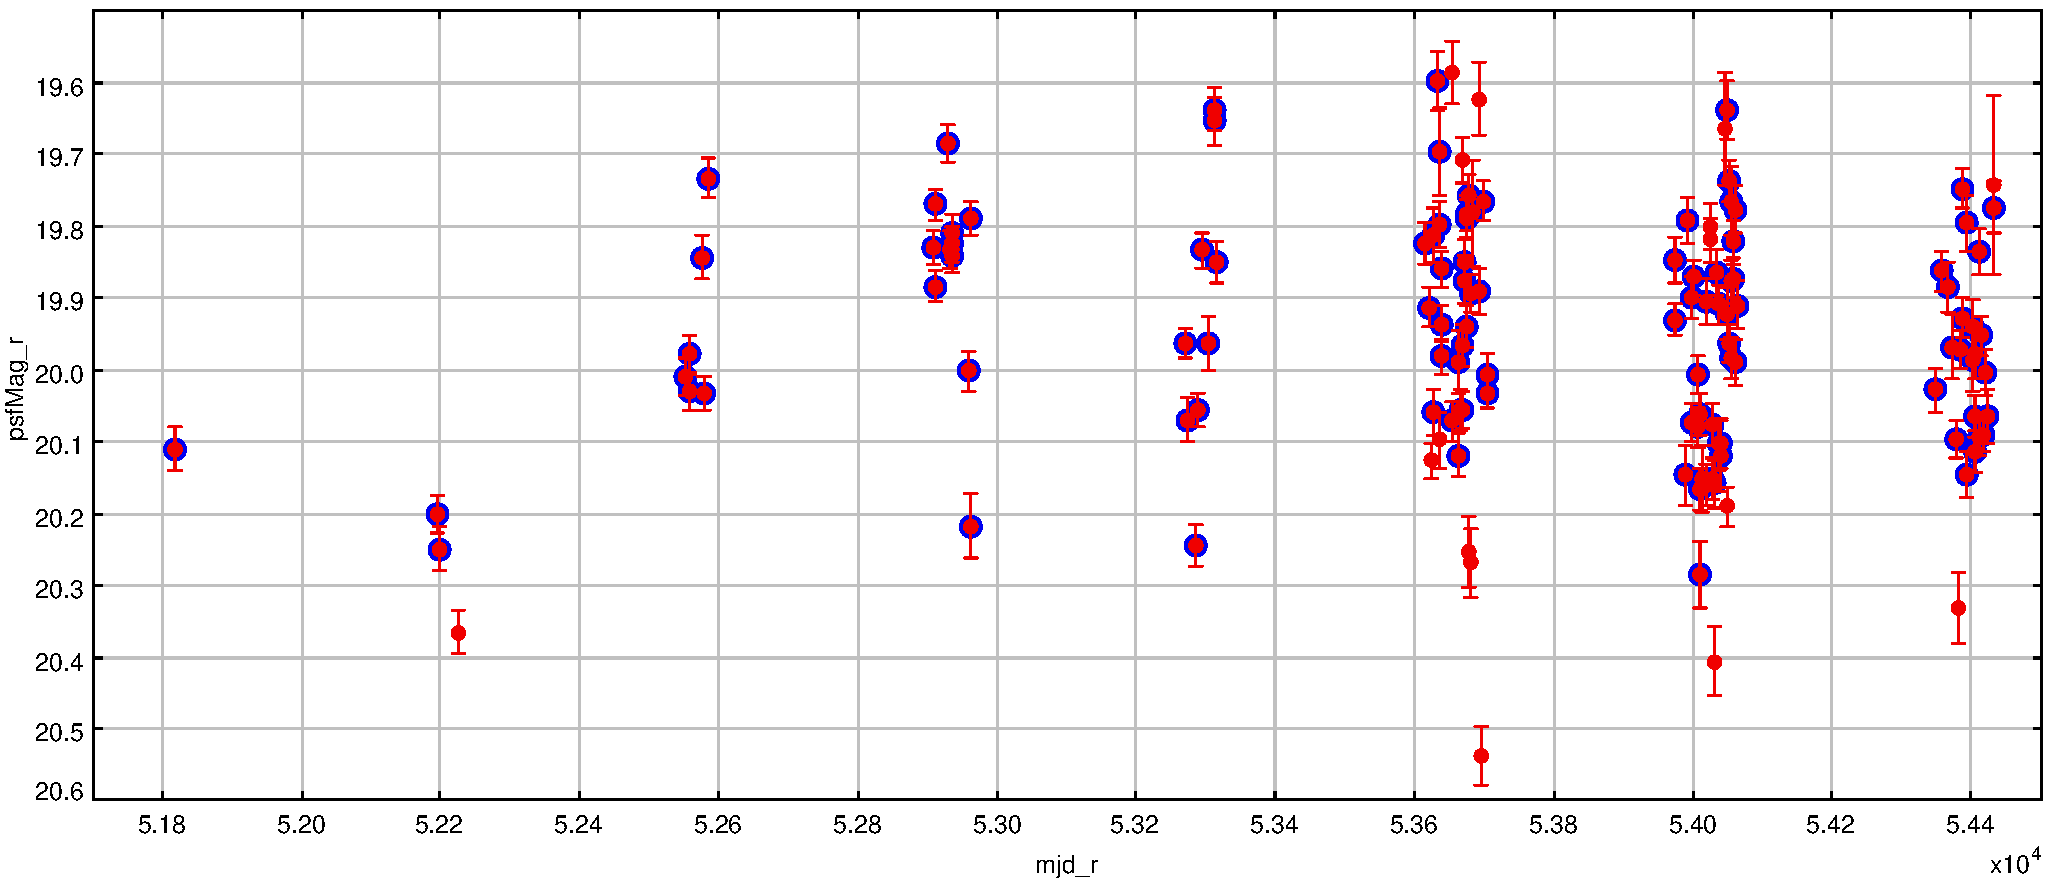
\includegraphics[width=0.90\textwidth]{figs/S82lens587731185128308933_rLC_all.pdf}
\textit{\caption[...]{The photometric r-band 'light curve' for the Stripe 82 lens \href{http://casjobs.sdss.org/dr7/en/tools/explore/obj.asp?id=587731185128308933}{ULAS J234311.93-005034.0} \citep{jackson08}. The messy light curve washes out the variability signal from the underlying intrinsic quasar variability of the two images, causing the object to fall outside the variability selection cut from \cite{schmidt10}. This might also be the reason that the 5 'personal favorites' also fail our variability cut ... and be an indication of a lens nature?}
\label{fig:lensLC}}
\end{figure} 
%====================================
%====================================



\subsection{sample}
The final list of objets for photometric follow-up is shown below (priority
IDs with less than 17 digits should be thought of as having zeros in front
(i.e. no spec and/or no H-band mag and/or
$\chi_\textrm{star}^2<\chi_\textrm{phot}^2$ smaller than 0.5).
\begin{verbatim}
# index   objid                priorityid          ra             dec          
  1       587730847424905311   28307024710390038   314.46866      0.10980109   
  2       588015508755775570   28223052419080255   53.20213       -0.3653704   
  3       587731172232135333   28198010123940667   313.38757      -1.0162246   
  4       587734305413726557   28184014016370613   331.25497      0.52302201   
  5       587731512076075139   28164010819880032   35.201385      -0.47599432  
# index   objid                priorityid          ra             dec          
  6       587731513141559419   18376002311520013   16.2803823     0.41126949   
  7       588015509270495301   18319003126990003   2.56871133     0.20768695   
  8       587731186191237426   18319000828350003   331.03966347   -0.13770241  
  9       587731185662951500   18318021115240003   350.60691496   -0.46557767  
  10      587731185668194449   18312148931960003   2.59227832     -0.61700182  
  11      587730845818683704   18295000427890024   324.52846301   -1.13821544  
  12      588015507663683725   18276000507450250   11.31436324    -1.22159835  
  13      587731513145950268   18266007922250005   26.33675498    0.27844314   
  14      587731186202181850   18266000528230004   356.07654605   -0.14918738  
  15      587731186191106371   18264001027670009   330.79126123   -0.05476811  
  16      587731513695338778   18261000131170005   54.98491555    0.74094738   
  17      587731173843141315   18260000821680100   314.30536647   0.34196573   
  18      587731185666883640   18259022710160003   359.63513674   -0.54471111  
  19      587731513142673569   18258037111630003   18.90717437    0.34129864   
  20      587731187282935899   18249010323490004   12.02523834    0.77324401   
  21      587734303265521855   18244001226760003   329.47267164   -1.06699208  
  22      587731512069193830   18243016610500005   19.43621533    -0.50922581  
  23      587731513151586516   18238000035570008   39.22277877    0.40554146   
  24      587731511533633570   18237034314450006   22.42771056    -0.93304814  
  25      587731185116512658   18234000741220007   328.87087805   -0.86667065  
# index   objid                priorityid          ra             dec          
  26      587731185649844313   18289020220100019   320.67921931   -0.44823529  
  27      587731511548051657   18253000216713650   55.41522299    -0.9305844   
  28      587731511546413317   18150003520218300   51.59492157    -0.93060182  
  29      587730846887903261   8499000128010022    314.13792241   -0.32785762  
  30      587731513160499326   8368000721000278    59.49807353    0.21947222   
  31      587730847426937208   8363002221232200    319.20750215   0.18337412   
  32      588015509287076033   8358000821573900    40.5198754     0.13737578   
  33      587730846349656754   8350000134780400    311.0127548    -0.79229016  
  34      588015508744175661   8347002021340077    26.68992988    -0.30831431  
  35      588015510357606468   8343000228350136    33.08143591    0.97796328   
  36      587731513147785320   8339012421004300    30.5985167     0.31552293   
  37      587731513154797670   8336000821460041    46.48088427    0.36476759   
  38      587731512081514575   8326000515921333    47.57941789    -0.51895294  
  39      588015508208287957   8324000518520229    28.98552678    -0.8355823   
  40      587731185665179793   8306001220100875    355.76767567   -0.56417785  
  41      587734304878362816   8304000518520106    334.6089575    0.00358132   
  42      587731185661313236   8298000427897600    346.95847999   -0.50080682  
  43      587734304876396906   8285000415360045    330.20091782   0.09621753   
  44      587731511548838044   8284000215920010    57.13492648    -0.90031382  
  45      587734303802589408   8281002718523400    329.92277966   -0.77728322  
  46      587730847964332566   8279000315920278    320.40150042   0.56287791   
  47      588015508733624396   8276000216830438    2.53962976     -0.24894871  
  48      587731513160564968   8272000134903300    59.64656503    0.27817405   
  49      587731513697370521   8272000133881600    59.62061801    0.71050234   
  50      587734304875151606   8267000916150076    327.31382478   0.05119274   
  51      587731186733351039   8263002920447000    342.94927851   0.27793996   
  52      587731173841633816   8257002517620065    310.93381413   0.29493685   
  53      587731511549755695   8256000035126700    59.32960586    -1.00863174  
  54      587731513146081322   8254000615818500    26.69367325    0.39718462   
  55      588015509295268047   8247001217731017    59.21982537    0.12025366   
  56      588015507679936910   8245000413100273    48.43967501    -1.11547378  
  57      588015508221526343   8242000035240633    59.22716971    -0.72473727  
  58      588015509829779619   8240000215920169    53.78393564    0.47095532   
  59      587731511549493558   8240000134780173    58.63604141    -0.96547939  
  60      587731513160368403   8240000115360278    59.34605541    0.37801641   
  61      587731513149292677   8238000626540429    33.97354788    0.30745282   
  62      587731174381257370   8235000128127500    317.19443538   0.69220297   
  63      587730846886200909   8231000134900039    310.2969856    -0.22724373  
  64      587731513160564920   8228000034446700    59.65532312    0.36049748   
  65      587731513159975206   8226000134902267    58.43069538    0.33322058   
  66      588015508758397216   8226000034223200    59.11949103    -0.32329802  
  67      587734305412023026   8224000128120385    327.37109131   0.44621311   
  68      587731513159254241   8223000115473750    56.68708635    0.29622657   
  69      587731512086233546   8221000134906700    58.43803043    -0.53917304  
  70      587731513697042711   8220000141563350    58.87042553    0.67164754   
  71      587731512620548263   8219001416040425    52.54430662    -0.12571542  
  72      588015508193476871   8216000215920025    355.14216357   -0.74241339  
  73      587734305413661075   8212000416043250    331.00978471   0.42840843   
  74      587731513696321913   8210000134677200    57.1507037     0.69316917   
  75      587731512623104241   8209000115367000    58.41231406    -0.1021376   
  76      587731186203492548   8208000915470690    359.03272438   -0.13177073  
  77      588015507684786413   8207000115243100    59.49140514    -1.15768651  
  78      587731513154404751   8207000034110127    45.6382539     0.22525097   
  79      588015509806383318   8204000115360600    0.28134042     0.4404782    
  80      587731513159254285   8203000033657000    56.65311597    0.29550801   
  81      588015508758462676   8202000139873200    59.29353774    -0.29290781  
  82      587731512606851264   8201000115920730    21.18745158    -0.11899497  
  83      587731185653252727   8199000216710689    328.45076296   -0.49241653  
  84      588015508758462628   8196000720100012    59.38294514    -0.37495876  
  85      588015509831877068   8196000135240663    58.56111494    0.53564565   
  86      587731186726470168   8194000115360226    327.30862891   0.39783338   
  87      588015509825126671   8194000034333850    43.17498245    0.44043288   
  88      587731512086757648   8193000134446700    59.53757794    -0.50116709  
  89      588015508221460870   8192000044270900    58.98617812    -0.67585814  
  90      587734304339198809   8191000215470253    329.47084958   -0.40949876  
  91      588015507656409329   8191000134330775    354.67771397   -1.24065329  
  92      588015508207828998   8189000417730700    27.82587352    -0.79557914  
  93      587731513690292410   8189000127220286    43.32938887    0.81778804   
  94      587731513697304999   8189000115476700    59.3975202     0.67716281   
  95      588015510358458608   8188000115920427    35.04298921    1.01970783   
  96      587731511549559087   8188000115363400    58.87078743    -0.91100662  
  97      587731513964495202   8187000035123700    56.62906936    0.66774582   
  98      587731512623628539   8185000115366700    59.49679676    -0.13496326  
  99      588015509801664770   8185000115360610    349.48809333   0.5748918    
  100     587730846352409836   8184000035800325    317.38168232   -0.70777331  
  101     588015509281964328   8182000315360012    28.77326408    0.05285465   
  102     587731185671930420   8181000015360888    11.19816342    -0.58054176  
  103     587731513159516396   8180000215920159    57.25131914    0.36703432   
  104     587734304344113619   8180000213100060    340.67748562   -0.30502157  
  105     588015508753285444   8179000140882600    47.42559754    -0.24083923  
  106     588015509831745823   8179000135461017    58.25954888    0.58006054   
  107     588015508215234812   8178000034900438    44.82696638    -0.75716066  
  108     588015509289632089   8177000516710259    46.34723584    0.08097379   
  109     587731187265372311   8177000215810700    331.956594     0.68745054   
  110     587731174380471444   8176000216710172    315.39371955   0.79036522   
  111     587731512623431999   8176000210615500    59.15970642    -0.20052501  
  112     588015509832335717   8176000134670091    59.6614699     0.43801391   
  113     588015509273117045   8176000035013300    8.54317644     0.1391726    
  114     587731511545299205   8175000135690938    49.02232469    -1.03599468  
  115     588015507684524310   8175000035123050    58.92980723    -1.21081217  
  116     588015508732051682   8174000315470763    358.93532029   -0.32688323  
  117     588015508742144300   8173000134902267    21.99672073    -0.34916142  
  118     587731513150341377   8172000215810231    36.31586499    0.30134035   
  119     587731512080531877   8172000133200017    45.35428357    -0.60279308  
  120     587731513160040734   8171000033200610    58.54230901    0.31968225   
  121     588015509295137044   8170000035805000    58.8276544     0.0845214    
  122     587731511537041702   8169000215470480    30.22219146    -0.89729309  
  123     587731512622055894   8167000034447300    55.9861992     -0.09513339  
  124     587734303802917334   8166000714570037    330.69295078   -0.6965352   
  125     588015508219035851   8166000028351375    53.52409235    -0.71314309  
  126     587731512623366502   8165000234676600    59.03555463    -0.0536828   
  127     588015508196950177   8164000128460196    3.10111897     -0.80628799  
  128     587730847960924753   8162000134783200    312.63502143   0.59111235   
  129     587731513696584077   8162000034227600    57.78296332    0.72911735   
  130     588015509285896326   8161008319880010    37.79431145    0.06472738   
  131     587731186728173973   8161000127220667    331.23216805   0.28880648   
  132     587731512086757696   8161000114682167    59.62101297    -0.57216759  
  133     588015509814444402   8160003020890075    18.76360994    0.57122385   
  134     587734303269519654   8158005121460067    338.69686764   -1.20383202  
  135     587731512086167921   8158000415367000    58.21106073    -0.45101632  
  136     588015508740178139   8158000115360146    17.50382877    -0.30823647  
  137     588015509822505291   8157000420440381    37.13839876    0.56612756   
  138     587730847964529079   8157000315701267    320.75744239   0.42708932   
  139     588015508757676279   8157000215477100    57.53712747    -0.40963053  
  140     587731187266683333   8157000215240457    334.86468084   0.70790628   
  141     588015508752760943   8156015113100114    46.37135451    -0.29464218  
  142     588015507676070208   8156003817280013    39.55680949    -1.05401309  
  143     588015508221395275   8156000133773000    58.92255671    -0.78147716  
  144     587731512623497546   8156000033990300    59.25726379    -0.11821027  
  145     588015508756955387   8155000028460800    55.9546446     -0.40566588  
  146     588015508205863402   8154000033200097    23.3779105     -0.82782683  
  147     587731513159909592   8153000035123350    58.15865136    0.29197695   
  148     587731173845566506   8153000034330100    319.84713021   0.36313935   
  149     588015508221198797   8152000135126200    58.41196708    -0.72514849  
  150     587731187283394828   8152000113100900    13.13491772    0.76231608   
  151     588015507675939143   8152000031400433    39.33287343    -1.17832153  
  152     587731185654301192   8151000115470387    330.82967835   -0.43041495  
  153     588015509831680310   8151000115366700    58.13388328    0.60079205   
  154     587731513692520692   8150000221570161    48.4386123     0.66266778   
  155     588015509830238543   8149000127890722    54.87987994    0.48490571   
  156     587731187264258598   8148000115366900    329.382684     0.77930676   
  157     588015508221198760   8148000034901575    58.38595437    -0.74178315  
  158     587731513678168565   8147000128123650    15.7209482     0.72841514   
  159     587731512067686775   8146000215470295    16.05285909    -0.60336083  
  160     587734305417003445   8146000113100172    338.75240093   0.50843897   
  161     587731511548903804   8146000034780067    57.36230746    -0.92830303  
  162     588015509295268053   8146000034443100    59.10137589    0.14827754   
  163     587731187265831421   8144003419650300    332.9891467    0.74197576   
  164     588015509294940513   8144000133996600    58.38961073    0.0454719    
  165     587731511543595137   8144000133543900    45.20732779    -1.03442186  
  166     588015507683344593   8144000128010232    56.19775318    -1.11299607  
  167     588015509282947766   8143000034900582    31.09223502    0.16831282   
  168     588015507668861362   8142000035242333    23.11504517    -1.06607055  
  169     587731187268518233   8142000034440536    339.15757513   0.73278811   
  170     587731186187437241   8141000134670929    322.36493861   -0.13575693  
  171     587731511536124240   8140000115580673    28.20391077    -0.85450959  
  172     587731511549821176   8138001120216100    59.41236144    -0.94732236  
  173     587731185659412865   8137000415366800    342.50746258   -0.45843835  
  174     587730846891967208   8137000128120210    323.55974089   -0.22850165  
  175     587731186197397858   8136002917500185    345.17370897   -0.0977527   
  176     588015509293957343   8136000914790164    56.16460338    0.02040898   
  177     588015509295268135   8136000134561450    59.21231254    0.13272463   
  178     587731512622776674   8136000035016900    57.62191645    -0.15901664  
  179     587731185122214405   8135000034112200    341.86071469   -0.96675579  
  180     588015509831549251   8134000133993300    57.78773369    0.43516396   
  181     587730847963545622   8134000033880473    318.48788942   0.47863715   
  182     587730846887970055   8130001113320174    314.32077642   -0.21608928  
  183     587731512623169818   8129000115361050    58.54077913    -0.1976403   
  184     588015509291532776   8128000128351520    50.64092826    0.13759007   
  185     587730845813506750   8128000028573050    312.67490363   -1.18092076  
  186     588015508221526333   8127000120440181    59.21363277    -0.78694037  
  187     588015508758331647   8127000115360336    59.09825222    -0.35265251  
  188     587731512619761746   8125000415241114    50.78253112    -0.132287    
  189     588015508757938481   8124000134670325    58.08702142    -0.24712597  
  190     587731512622907834   8124000035353550    57.97864625    -0.14892255  
  191     588015509276459308   8123000034566800    16.16955676    0.16425819   
  192     587730845814031429   8122000115360013    313.94746283   -1.21329413  
  193     587731513697108201   8122000032750210    58.94153187    0.6869974    
  194     587731185658233209   8120000415920064    339.93955905   -0.59000409  
  195     587731186738463064   8118000215923700    354.70007709   0.24482354   
  196     588015507684786462   8118000120780052    59.44389862    -1.12770186  
  197     588015509270299092   8118000115470580    2.1841057      0.10122366   
  198     587731513155060070   8118000028468300    47.10516626    0.39018651   
  199     587731513159975183   8117000217280103    58.39791532    0.21880155   
  200     588015510099394944   8116001514340914    56.54405526    0.51627307   
  201     587734304877969870   8116000115360049    333.68423737   0.16727162   
  202     588015508751974574   8116000113100137    44.45757273    -0.35229808  
  203     587731512086561000   8114000134110613    59.12003661    -0.54335662  
  204     587731513691603319   8113001416830037    46.37468326    0.66047545   
  205     587730845813834031   8113000127560675    313.49904748   -1.08403159  
  206     588015508757676518   8112000134786600    57.54836709    -0.27533476  
  207     587731512623628749   8112000035570473    59.54308442    -0.08516352  
  208     587731512618451022   8110000115360142    47.81240222    -0.14849066  
  209     588015509832335992   8110000034561325    59.66169679    0.48440177   
  210     588015509831549263   8109000215815900    57.79905328    0.47970973   
  211     588015507684524489   8109000135240307    58.9163517     -1.07868629  
  212     587731186209063393   8109000134781233    11.79211349    -0.13265296  
  213     587731512086167959   8109000134226800    58.24371333    -0.5885599   
  214     588015508221722930   8109000133202700    59.56556       -0.74982017  
  215     587731185657905570   8108001221000192    339.09666898   -0.57223538  
  216     588015508758462714   8108000034445400    59.35810524    -0.22867327  
  217     587731511549886785   8107000135690073    59.51014178    -0.91844885  
  218     588015508758069546   8106000136031967    58.42458855    -0.40143638  
  219     587731512618516744   8103000214910177    47.89440832    -0.06383865  
  220     587731511549624656   8101000213890076    58.95356462    -0.89516213  
  221     588015509294678422   8101000133990527    57.81113082    0.12076061   
  222     587731512080597248   8100003618294200    45.45703902    -0.43151794  
  223     588015508758593851   8100000311400967    59.6920345     -0.37965086  
  224     588015509824929832   8100000115247600    42.66718653    0.52500656   
  225     588015509832204597   8097000131060232    59.26932896    0.60004572   
  226     587731512086298830   8095000618180037    58.4599219     -0.58955698  
  227     588015507659816992   8095000327330052    2.48283581     -1.05976892  
  228     587731513159516499   8094000115360270    57.34759756    0.2660508    
  229     588015508196884653   8089000818290235    2.85310149     -0.70058369  
  230     587731512086626571   8081000133543000    59.29297582    -0.54043985  
  231     588015507684524335   8078000133655600    58.81541874    -1.1031397   
  232     588015508755775915   8078000035120986    53.13603196    -0.29591489  
  233     588015508758331616   8075000215700757    59.00819477    -0.38118571  
  234     588015509811494927   8072000715923100    12.00119588    0.47559751   
  235     587731512623104322   8069000519880039    58.39275232    -0.19519354  
  236     588015508758331425   8067000134332600    59.04065796    -0.36535815  
  237     587731513160171748   8063000130830146    58.83232411    0.37507007   
  238     588015508221395117   8062000134440950    58.9062555     -0.8361573   
  239     587731511549755668   8060000126990076    59.28393358    -0.9688947   
  240     588015508757872848   8027000426310026    57.99023391    -0.2590211   
  241     587731187267403918   437416710057        336.59038795   0.68109403   
  242     587731186729746587   6216831117          334.84010537   0.2521135    
  243     587731511544250723   3015920159          46.66491808    -0.97092109  
  244     587731185114284838   2213210129          323.71150472   -0.96575017  
  245     587731185118937554   1914230161          334.28517098   -1.02085116  
  246     587730845814424771   1722360116          314.82437057   -1.08159925  
  247     587731512622186720   1518520043          56.34806959    -0.13073886  
  248     587731185127391596   1518290047          353.59757545   -0.91635395  
  249     587731512085840285   1317280347          57.48801599    -0.60855684  
  250     587731186210177284   1315240767          14.25313528    -0.12001091  
  251     587731512073191781   1314340140          28.65331511    -0.4788035   
  252     587731185121493030   1117730165          340.1392284    -0.94759052  
  253     587731185130471520   1112310411          0.74298145     -0.94751432  
  254     587734303271813439   1014340022          343.97503168   -1.16868639  
  255     588015509274820803   917500025           12.46657918    0.14251553   
  256     587731186728174168   916040373           331.22892868   0.27209253   
  257     587731513153421521   818410043           43.44135089    0.40701439   
  258     588015508210319585   815362467           33.60361815    -0.73092825  
  259     588015509801664769   719650045           349.48424718   0.42292919   
  260     588015508192231648   718290103           352.29610075   -0.77202698  
  261     587731186193858823   715920920           337.09326925   -0.01025064  
  262     587731172235150025   713100142           320.25195566   -0.96135897  
  263     587730847427461228   618180067           320.32099531   0.19603973   
  264     587730847425954816   520550020           316.88496151   0.0335037    
  265     587730846891049682   515360209           321.38626896   -0.40148726  
  266     587731185130471695   422590235           0.70874782     -0.90549417  
  267     587731513141821725   420783750           16.94982962    0.22596645   
  268     588015509832073495   420780039           58.95248529    0.48061624   
  269     587731512622186716   420210029           56.28150337    -0.01963803  
  270     587734304340574554   418290021           332.48699145   -0.23027411  
  271     587734303268733397   416150020           336.95387741   -1.05208907  
  272     588015509264007352   327675500           347.74559764   0.11967978   
  273     588015509831877162   318290159           58.63578097    0.58965237   
  274     587734303806193738   317280571           338.20131333   -0.77751735  
  275     588015507667484948   315472500           20.00795148    -1.18337907  
  276     587731172234167101   315472400           318.05520514   -1.02542921  
  277     587731511549624693   313105900           59.02204932    -0.99765201  
  278     588015508758462723   312990210           59.37301732    -0.23504135  
  279     587731185655546325   312990073           333.70464196   -0.44467872  
  280     588015508758397323   238510042           59.13648366    -0.40846632  
  281     587731513696125009   234780957           56.76783232    0.77493197   
  282     587730846889477102   226880223           317.76611171   -0.34721413  
  283     588015509831811429   221460090           58.46974851    0.54565461   
  284     588015508758135063   218290032           58.58206157    -0.2561638   
  285     587731512623366469   217390140           58.99851515    -0.01823615  
  286     587731512079024454   215474100           41.90059018    -0.52164718  
  287     587730847962956757   215470205           317.2138254    0.60682516   
  288     587731513160237331   215361020           59.01328764    0.40578424   
  289     587730847965905723   215360600           323.91700036   0.5132631    
  290     587731186726535718   215360218           327.38549825   0.32574879   
  291     587730847424316792   215360174           313.21345684   0.0988313    
  292     587731512616878324   215240102           44.21197152    -0.11983943  
  293     588015507681247555   214910276           51.41708085    -1.23302861  
  294     587731186191434269   214790027           331.53724989   -0.19070039  
  295     587730847429362667   213100242           324.72355463   0.14186963   
  296     588015507684720966   211292100           59.30315802    -1.23050756  
  297     587731185658560906   210841100           340.60464893   -0.43566145  
  298     588015509832073530   210390107           59.0256913     0.55715604   
  299     587731513160106176   210280027           58.6220605     0.39043623   
  300     587734303808291111   140320467           342.95493691   -0.71315262  
  301     587734304878232115   135690289           334.3519734    0.17554752   
  302     587731512082563511   135240592           49.98459438    -0.60565936  
  303     587730846887707889   134900143           313.82778327   -0.21729537  
  304     587731172231874007   134900050           312.85511792   -0.96543046  
  305     587731513695404423   134670492           55.07920111    0.70262214   
  306     587731174380209520   134560097           314.75899194   0.64370938   
  307     588015507681051066   134441460           50.99881998    -1.08437795  
  308     587731511548838221   134440421           57.21030448    -0.92032308  
  309     587731186194514254   134440268           338.48704867   -0.1181148   
  310     587731513697042683   134336500           58.84251622    0.762885     
  311     587731174381585239   134330469           317.95734363   0.74943607   
  312     588015508207108378   134220106           26.23686833    -0.74402563  
  313     587731511549886827   134220040           59.55122674    -0.88869329  
  314     587731187266290330   134112233           334.02690686   0.77361557   
  315     587730846887314833   134111200           312.83872757   -0.25413837  
  316     587734304881705555   134110814           342.30151006   0.05289905   
  317     587731513694224936   133990189           52.44063488    0.64227716   
  318     588015508758135024   133881160           58.51791095    -0.35175974  
  319     588015509295202668   133775900           59.08122966    0.15070171   
  320     587731513697042890   133770638           58.88202348    0.65490354   
  321     587730846617306966   133770130           309.24227336   -0.76428664  
  322     588015508729823549   133541260           353.87573253   -0.2531515   
  323     587731513695797659   133320971           55.96871496    0.66911208   
  324     588015508221526439   132754600           59.14067097    -0.67243301  
  325     587731513154208026   131178300           45.17140294    0.3579937    
  326     588015508735394046   128356500           6.66337255     -0.33304229  
  327     588015508738736373   128013400           14.23820074    -0.31963798  
  328     587731512620613660   127898200           52.62931518    -0.13111995  
  329     587731513151586591   127892267           39.17801341    0.28468093   
  330     587731187273826547   127780139           351.2024931    0.83324067   
  331     587731172231939346   127565800           312.96177701   -0.95326722  
  332     587731172231742759   127220379           312.46055444   -0.89263362  
  333     587731511543726225   126430067           45.49038935    -1.03302436  
  334     587731513697108346   120670733           58.94019153    0.78251187   
  335     588015508758266234   118291100           58.84111086    -0.34850862  
  336     587731512083546440   115474050           52.17264937    -0.48412451  
  337     587731512606654685   115470600           20.7649507     -0.08188066  
  338     587731172234888035   115470262           319.69687143   -0.97570754  
  339     587731513692914188   115368100           49.46444186    0.64395283   
  340     587731512622514473   115367300           56.96576525    -0.11798873  
  341     587731512608228002   115362700           24.415049      -0.17126901  
  342     587731513159254334   115361750           56.67840691    0.31365821   
  343     587730847424381440   115361360           313.36771549   0.00711525   
  344     587731172768678368   115360667           312.60967442   -0.5915194   
  345     587731172231087742   115360458           311.09561734   -1.00064818  
  346     587730846352082003   115360373           316.59219363   -0.69881352  
  347     587731187261309729   115360311           322.64291345   0.64291372   
  348     587731513680199890   115360196           20.37960931    0.6721281    
  349     587731185113170729   115360169           321.22160808   -0.90579481  
  350     587734303265981141   115360165           330.62960177   -1.23140959  
  351     588015507674431778   115360120           35.82194609    -1.11599079  
  352     587731512609210590   115360118           26.57495542    -0.03742235  
  353     587731512069718496   115243950           20.71033271    -0.59590878  
  354     588015508202193431   115243400           15.06448416    -0.72462555  
  355     588015508201406848   115240176           13.2086915     -0.72137367  
  356     588015508757610871   115240077           57.32860447    -0.24738298  
  357     587731512623563042   113101525           59.36930925    -0.08859901  
  358     587731511548051859   113101400           55.45087936    -0.94333781  
  359     587731513160237283   113101325           58.94004       0.35657832   
  360     587731174109349704   113100320           309.22172179   0.3661501    
  361     587731187263210022   113100089           326.94849039   0.78010401   
  362     588015507666567534   112991280           17.92123597    -1.21306035  
  363     587731513160171884   42240325            58.86778071    0.33673866   
  364     587731511548641679   35127400            56.68616685    -0.84818492  
  365     587731512069063001   35120655            19.12545604    -0.62085157  
  366     588015507676004672   35011875            39.42723664    -1.1668912   
  367     587731185671275025   34900493            9.68746488     -0.58190564  
  368     588015509832139206   34781425            59.17290647    0.56539935   
  369     588015509832073424   34675800            59.09073073    0.59449696   
  370     587731513696649696   34221750            57.97837595    0.81783323   
  371     587731511548707261   34117200            56.9435402     -1.01500012  
  372     587731512623628664   33993100            59.62170378    -0.13729464  
  373     587734304875217346   33991140            327.3800419    0.14956247   
  374     588015508203569700   33886800            18.16363029    -0.80049918  
  375     587731185115595561   33777100            326.72253779   -1.04220844  
  376     587731513696649648   33657200            57.94241462    0.80756885   
  377     588015507659686317   33540871            2.17255035     -1.18011633  
  378     588015508457718061   33540775            345.52546611   -0.73057677  
  379     588015508740047285   33430400            17.26438836    -0.37962746  
  380     587731512616747476   33324300            43.89694645    -0.08795348  
  381     587730845814424960   33200022            314.79292287   -1.19030964  
  382     588015508758462607   32862350            59.31604189    -0.25448186  
  383     587731513688064337   28574150            38.27116763    0.82463903   
  384     587731174377980102   28351733            309.63789234   0.81011137   
  385     587731514219561037   28350500            26.10617414    1.1587008    
  386     587731172230694402   28120886            310.19145883   -0.98470423  
  387     588015509295137099   14680433            58.9267184     0.09443982   
\end{verbatim}

%======================================================================

\begin{thebibliography}{99}

\bibitem[Schmidt et al.(2010)]{schmidt10}
Schmidt, K. B., Marshall, P. J., Rix, H.-W., Jester, J., Hennawi, J. F., \& Dobler, G., 2010, ApJ, 714, 1194 

\bibitem[Oguri \& Marshall(2010)]{oguri10}
Oguri, M., \& Marshall, P. J., 2010, MNRAS, 405, 2579

\bibitem[Schneider et al.(2007)]{schneider07}
Schneider, D. P. et al., 2007, AJ, 134, 102

\bibitem[Lacki et al.(2008)]{lacki08}
Lacki, B. C. et al., 2008, ApJ, 698, 428

\bibitem[Jackson et al.(2008)]{jackson08}
Jackson, N. et al., 2008, MNRAS 387, 741

\bibitem[Hennawi et al.(2010)]{hennawi10}
Hennawi, J. F., et al., 2010, ApJ, 719, 1672
\end{thebibliography}

%======================================================================
\end{document}
